% Options for packages loaded elsewhere
\PassOptionsToPackage{unicode}{hyperref}
\PassOptionsToPackage{hyphens}{url}
%
\documentclass[
]{book}
\usepackage{amsmath,amssymb}
\usepackage{lmodern}
\usepackage{iftex}
\ifPDFTeX
  \usepackage[T1]{fontenc}
  \usepackage[utf8]{inputenc}
  \usepackage{textcomp} % provide euro and other symbols
\else % if luatex or xetex
  \usepackage{unicode-math}
  \defaultfontfeatures{Scale=MatchLowercase}
  \defaultfontfeatures[\rmfamily]{Ligatures=TeX,Scale=1}
\fi
% Use upquote if available, for straight quotes in verbatim environments
\IfFileExists{upquote.sty}{\usepackage{upquote}}{}
\IfFileExists{microtype.sty}{% use microtype if available
  \usepackage[]{microtype}
  \UseMicrotypeSet[protrusion]{basicmath} % disable protrusion for tt fonts
}{}
\makeatletter
\@ifundefined{KOMAClassName}{% if non-KOMA class
  \IfFileExists{parskip.sty}{%
    \usepackage{parskip}
  }{% else
    \setlength{\parindent}{0pt}
    \setlength{\parskip}{6pt plus 2pt minus 1pt}}
}{% if KOMA class
  \KOMAoptions{parskip=half}}
\makeatother
\usepackage{xcolor}
\IfFileExists{xurl.sty}{\usepackage{xurl}}{} % add URL line breaks if available
\IfFileExists{bookmark.sty}{\usepackage{bookmark}}{\usepackage{hyperref}}
\hypersetup{
  pdftitle={An Open Geomatics Textbook},
  pdfauthor={UBC},
  hidelinks,
  pdfcreator={LaTeX via pandoc}}
\urlstyle{same} % disable monospaced font for URLs
\usepackage{longtable,booktabs,array}
\usepackage{calc} % for calculating minipage widths
% Correct order of tables after \paragraph or \subparagraph
\usepackage{etoolbox}
\makeatletter
\patchcmd\longtable{\par}{\if@noskipsec\mbox{}\fi\par}{}{}
\makeatother
% Allow footnotes in longtable head/foot
\IfFileExists{footnotehyper.sty}{\usepackage{footnotehyper}}{\usepackage{footnote}}
\makesavenoteenv{longtable}
\usepackage{graphicx}
\makeatletter
\def\maxwidth{\ifdim\Gin@nat@width>\linewidth\linewidth\else\Gin@nat@width\fi}
\def\maxheight{\ifdim\Gin@nat@height>\textheight\textheight\else\Gin@nat@height\fi}
\makeatother
% Scale images if necessary, so that they will not overflow the page
% margins by default, and it is still possible to overwrite the defaults
% using explicit options in \includegraphics[width, height, ...]{}
\setkeys{Gin}{width=\maxwidth,height=\maxheight,keepaspectratio}
% Set default figure placement to htbp
\makeatletter
\def\fps@figure{htbp}
\makeatother
\setlength{\emergencystretch}{3em} % prevent overfull lines
\providecommand{\tightlist}{%
  \setlength{\itemsep}{0pt}\setlength{\parskip}{0pt}}
\setcounter{secnumdepth}{5}
\usepackage{booktabs}
\ifLuaTeX
  \usepackage{selnolig}  % disable illegal ligatures
\fi
\usepackage[]{natbib}
\bibliographystyle{apalike}

\title{An Open Geomatics Textbook}
\author{UBC}
\date{2021-07-06}

\begin{document}
\maketitle

{
\setcounter{tocdepth}{1}
\tableofcontents
}
\hypertarget{preface}{%
\chapter*{Preface}\label{preface}}
\addcontentsline{toc}{chapter}{Preface}

This is the very first part of the book, which will eventually include the textbook's introduction. For now, here's some useful info for you:

\hypertarget{contacts}{%
\section{Contacts}\label{contacts}}

Paul Pickell, \href{mailto:paul.pickell@ubc.ca}{\nolinkurl{paul.pickell@ubc.ca}}\\
Evan Thornberry, \href{mailto:evan.thornberry@ubc.ca}{\nolinkurl{evan.thornberry@ubc.ca}}\\
Francois du Toit, \href{mailto:fdutoit@mail.ubc.ca}{\nolinkurl{fdutoit@mail.ubc.ca}}

\hypertarget{project-wiki}{%
\section{Project Wiki}\label{project-wiki}}

\href{https://github.com/ubc-geomatics-textbook/docs/wiki}{github.com/ubc-geomatics-textbook/docs/wiki}

\hypertarget{style-guide}{%
\section{Style Guide}\label{style-guide}}

\hypertarget{audience}{%
\subsection{Audience}\label{audience}}

\begin{enumerate}
\def\labelenumi{\arabic{enumi}.}
\tightlist
\item
  Audience is undergraduate of graduate student studying GIS, geomatics, and remote sensing with no prior knowledge in these subject areas (i.e., introductory).
\item
  Assume only first year-level knowledge (or equivalent concurrent learning) of mathematics, science (biology, chemistry, physics), and geography.
\item
  Assume a multicultural reader who is not necessarily familiar with Canadian geography and history.
\end{enumerate}

\hypertarget{general-style}{%
\subsection{General Style}\label{general-style}}

\begin{enumerate}
\def\labelenumi{\arabic{enumi}.}
\tightlist
\item
  Word spellings should follow \emph{The Oxford Canadian Dictionary (2 ed.)}.
\item
  Every chapter begins with 1-3 paragraphs of introductory text. The introductory text should be for general interest and not introduce any important terms that will be defined later in the chapter. The last sentence of this introductory text should summarize what students will learn.
\item
  Posing questions to readers is encouraged in all sections. For example, ``Have you ever wondered\ldots?'' ``How do you think X relates to Y?''
\item
  At every opportunity, authors should highlight Canadian examples of technology and science in geomatics. Examples of geomatics applications are highly encouraged in the Canadian context. For example, the following list of environmental management problems that are important to Canada should be discussed whenever possible:

  \begin{itemize}
  \tightlist
  \item
    Northern communities
  \item
    First Nations
  \item
    Climate change
  \item
    Boreal forest
  \item
    Endangered wildlife
  \item
    Freshwater management and ecosystems
  \item
    Fisheries
  \item
    Glaciers/ice monitoring
  \item
    Environmental justice
  \item
    Resource extraction
  \end{itemize}
\end{enumerate}

\hypertarget{learning-objectives}{%
\subsection{Learning Objectives}\label{learning-objectives}}

\begin{enumerate}
\def\labelenumi{\arabic{enumi}.}
\tightlist
\item
  Every chapter will have a numbered list of learning objectives that follow the introductory text.
\item
  There should be no period at the end of each listed learning objective.
\end{enumerate}

\hypertarget{summary}{%
\subsection{Summary}\label{summary}}

\begin{enumerate}
\def\labelenumi{\arabic{enumi}.}
\tightlist
\item
  All learning objectives should be addressed in the summary section.
\item
  The summary section should never introduce any new concepts, terms, or definitions and should never reference figures, tables, or equations.
\end{enumerate}

\hypertarget{key-terms}{%
\subsection{Key Terms}\label{key-terms}}

\begin{enumerate}
\def\labelenumi{\arabic{enumi}.}
\tightlist
\item
  Every chapter will have an alphabetical, but unnumbered list of key terms.
\item
  At first mention in the chapter text, key terms should be boldened and defined.
\end{enumerate}

\hypertarget{headings-and-labels}{%
\subsection{Headings and Labels}\label{headings-and-labels}}

\begin{enumerate}
\def\labelenumi{\arabic{enumi}.}
\tightlist
\item
  Chapter titles should use title-case and are numbered.
\item
  Chapter sub-titles are also numbered and in title-case. Sub-titles should go no lower than level 3 heading (i.e., 1.2.3).
\item
  Level 4 headings are not numbered, all letters are capitalized, and should only be used in special call-out boxes:

  \begin{itemize}
  \tightlist
  \item
    LEARNING OBJECTIVES
  \item
    REMEMBER THIS?
  \item
    YOUR TURN!
  \item
    CASE STUDY
  \end{itemize}
\end{enumerate}

\hypertarget{formulae}{%
\subsection{Formulae}\label{formulae}}

\begin{enumerate}
\def\labelenumi{\arabic{enumi}.}
\tightlist
\item
  Do not format formulae using Microsoft Word or LaTeX. Instead, formulae should be formatted with \href{https://bookdown.org/yihui/rmarkdown/markdown-syntax.html}{RMarkdown}.
\item
  Coordinates and Greek letters should always be formatted as formulae with RMarkdown.
\end{enumerate}

\hypertarget{units}{%
\subsection{Units}\label{units}}

\begin{enumerate}
\def\labelenumi{\arabic{enumi}.}
\tightlist
\item
  Standard International (SI) units should be used for the following:

  \begin{itemize}
  \tightlist
  \item
    Length = meter (m)
  \item
    Time = second (s)
  \item
    Amount of substance = mole (mole)
  \item
    Electric current = ampere (A)
  \item
    Temperature = Kelvin (K)
  \item
    Luminous intensity = candela (cd)
  \item
    Mass = Kilogram (kg)
  \end{itemize}
\item
  Angle degrees are preferred over radians (rad) when referencing geographic position.
\item
  Rates should be expressed with a dot operator and negative exponent rather than a divisor (e.g., m·s-1 or W·m-2).
\end{enumerate}

\hypertarget{numbers}{%
\subsection{Numbers}\label{numbers}}

\begin{enumerate}
\def\labelenumi{\arabic{enumi}.}
\tightlist
\item
  Scientific notation is the preferred way to represent large and small numbers and should use the × operator (not dot or asterisk) and be formatted as a formula (see Formulae): 1 × 102.
\item
  Scientific notation should be limited to four significant figures (e.g., 1.234 × 100) except for specific numbers where the precision is important or meaningful like the speed of light (2.99792458 × 108 m·s-1) or Planck's constant (6.62607004 × 10-34 J·s-1).
\item
  Constants (like above) and other physical variables should use \href{https://en.wikipedia.org/wiki/List_of_common_physics_notations}{common notations} (e.g., c for speed of light and h for Planck's constant) and be formatted as formulae (see Formulae).
\end{enumerate}

\hypertarget{dates-and-times}{%
\subsection{Dates and times}\label{dates-and-times}}

\begin{enumerate}
\def\labelenumi{\arabic{enumi}.}
\tightlist
\item
  The Gregorian calendar should be adopted for recent dates. In these cases, use Common Era (C.E.) to indicate dates after 0 A.D. and Before Common Era (B.C.E.) for dates before 0 A.D.

  \begin{itemize}
  \tightlist
  \item
    For specific recent dates, use the format ``20 February 2021'' and omit C.E.
  \item
    If many dates need to be summarized in a table, use the format ``DD-MM-YYYY''
  \end{itemize}
\item
  Times should be specified in either Local Standard Time (LST) or Coordinated Universal Time (UTC) using a 24-hour clock:

  \begin{itemize}
  \tightlist
  \item
    00:00 = 12 A.M. midnight LST
  \item
    12:00 = 12 P.M. noon LST
  \item
    23:00 = 11 P.M. LST
  \end{itemize}
\item
  For non-recent dates or when referring to geologic time scales, use the following:

  \begin{itemize}
  \tightlist
  \item
    Thousands of years before present = kilo annum (ka)
  \item
    Millions of years before present = mega annum (Ma)
  \item
    Billions of years = giga annum (Ga)
  \end{itemize}
\end{enumerate}

\hypertarget{tables}{%
\subsection{Tables}\label{tables}}

\begin{enumerate}
\def\labelenumi{\arabic{enumi}.}
\tightlist
\item
  Tables are numbered in the order that they appear in text and begin with the number of the chapter:

  \begin{itemize}
  \tightlist
  \item
    Table 1 in Chapter 1 = 1.1
  \end{itemize}
\item
  A short, descriptive caption should be written for a table.
\item
  Tables should only include information that is discussed or referenced in the chapter text.
\item
  Every table must be referenced in the chapter text.
\end{enumerate}

\hypertarget{code-blocks}{%
\subsection{Code blocks}\label{code-blocks}}

\begin{enumerate}
\def\labelenumi{\arabic{enumi}.}
\tightlist
\item
  Avoid code blocks in chapter text. Instead, try to place code blocks in TRY THIS! or CASE STUDY sections.
\item
  Only R code blocks should be embedded using \href{https://bookdown.org/yihui/rmarkdown/r-code.html}{RMarkdown}.
\end{enumerate}

\hypertarget{abbreviations}{%
\subsection{Abbreviations}\label{abbreviations}}

\begin{enumerate}
\def\labelenumi{\arabic{enumi}.}
\tightlist
\item
  Abbreviations are shortened form of a word or phrase and should be punctuated with periods:

  \begin{itemize}
  \tightlist
  \item
    e.g.
  \item
    Dr.
  \item
    Ph.D.
  \end{itemize}
\end{enumerate}

\hypertarget{initialisms}{%
\subsection{Initialisms}\label{initialisms}}

\begin{enumerate}
\def\labelenumi{\arabic{enumi}.}
\tightlist
\item
  Initialisms are the first letters of several words and should always be defined at first use in the chapter text regardless if the initialism is introduced and defined in an earlier chapter.
\item
  Do not introduce initialisms in figure or table captions or table text.
\item
  Except for the specific cases in this style guide, do not punctuate initialisms with periods:

  \begin{itemize}
  \tightlist
  \item
    AVHRR
  \item
    NDVI
  \end{itemize}
\end{enumerate}

\hypertarget{acronyms}{%
\subsection{Acronyms}\label{acronyms}}

\begin{enumerate}
\def\labelenumi{\arabic{enumi}.}
\tightlist
\item
  Acronyms are combinations of the first letters of several words and are pronounced as words. Acronyms should never be punctuated with periods.
\item
  Many satellites and remote sensing systems have acronyms that vary capitalization.
\item
  Following are some preferred acronyms:

  \begin{itemize}
  \tightlist
  \item
    Light Detection and Ranging = LiDAR
  \item
    Radio Detection and Ranging = RADAR
  \item
    Moderate Resolution Imaging Spectroradiometer = MODIS
  \end{itemize}
\end{enumerate}

\hypertarget{punctuation}{%
\subsection{Punctuation}\label{punctuation}}

\begin{enumerate}
\def\labelenumi{\arabic{enumi}.}
\tightlist
\item
  Use serial comma (Oxford comma) in lists: Yukon, Northwest Territories, and Nunavut.
\item
  Use italics for internal dialogue or when you infer what the reader might be thinking:

  \begin{itemize}
  \tightlist
  \item
    ``At this point, you might be wondering, \emph{why am I reading this sentence?}''
  \end{itemize}
\item
  Avoid the use of semi-colons.
\item
  Use and punctuate common Latin abbreviations with periods:

  \begin{itemize}
  \tightlist
  \item
    ``For example'' = exempli gratia (e.g.)
  \item
    ``That is'' = is est (i.e.)
  \item
    ``And other similar things'' = et cetera (etc.)
  \end{itemize}
\item
  Avoid phrases in parentheses () or brackets {[}{]}. Instead, place the phrase in a proper sentence.
\item
  Use single spaces between sentences.
\item
  Use double quotation marks for direct quotes, but avoid reproducing verbatim large texts. Paraphrasing with proper citation is preferred to direct quotation.
\item
  Bullet points are preferred over long lists in sentences.
\end{enumerate}

\hypertarget{citations}{%
\subsection{Citations}\label{citations}}

\begin{enumerate}
\def\labelenumi{\arabic{enumi}.}
\tightlist
\item
  Style should follow American Psychological Association (APA) format.
\item
  In-text references are encouraged where necessary, especially in case studies.
\item
  References and Recommended Readings section is placed at end of each chapter. Where possible, Recommended Readings should be populated with Open Educational Resources.
\end{enumerate}

\hypertarget{chapter-template}{%
\chapter{Chapter Title}\label{chapter-template}}

\textbf{Lorem ipsum dolor sit amet}, \emph{consectetur adipiscing elit.} Ut in dolor nibh. Lorem ipsum dolor sit amet, consectetur adipiscing elit. Praesent et augue scelerisque, consectetur lorem eu, auctor lacus. Fusce metus leo, aliquet at velit eu, aliquam vehicula lacus. Donec libero mauris, pharetra sed tristique eu, gravida ac ex. Phasellus quis lectus lacus. Vivamus gravida eu nibh ac malesuada. Integer in libero pellentesque, tincidunt urna sed, feugiat risus. Sed at viverra magna. Sed sed neque sed purus malesuada auctor quis quis massa.

\hypertarget{learning-objectives-1}{%
\subsubsection*{Learning Objectives}\label{learning-objectives-1}}
\addcontentsline{toc}{subsubsection}{Learning Objectives}

\begin{enumerate}
\def\labelenumi{\arabic{enumi}.}
\tightlist
\item
  Objective one
\item
  Objective two
\item
  Objective three
\end{enumerate}

\hypertarget{key-terms-1}{%
\subsection*{Key Terms}\label{key-terms-1}}
\addcontentsline{toc}{subsection}{Key Terms}

Ipsum lorem, Phasellus, sollicitudin, finibus

\hypertarget{first-section-header}{%
\section{First Section Header}\label{first-section-header}}

Lorem ipsum dolor sit amet, consectetur adipiscing elit. Ut in dolor nibh. Lorem ipsum dolor sit amet, consectetur adipiscing elit. Praesent et augue scelerisque, consectetur lorem eu, auctor lacus. Fusce metus leo, aliquet at velit eu, aliquam vehicula lacus. Donec libero mauris, pharetra sed tristique eu, gravida ac ex. Phasellus quis lectus lacus. Vivamus gravida eu nibh ac malesuada. Integer in libero pellentesque, tincidunt urna sed, feugiat risus. Sed at viverra magna. Sed sed neque sed purus malesuada auctor quis quis massa.

\begin{figure}
\centering
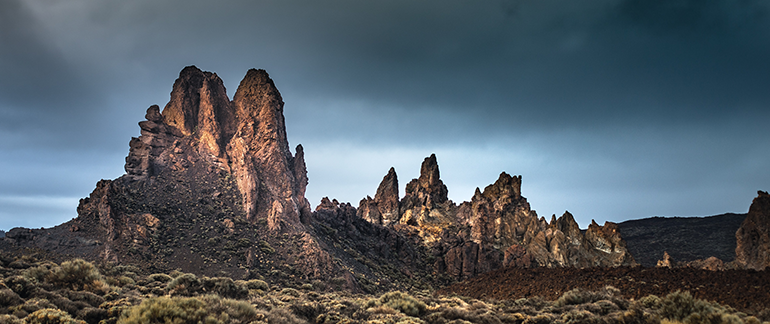
\includegraphics{images/01-image.png}
\caption{Figure caption text is also alt text.}
\end{figure}

Lorem ipsum dolor sit amet, consectetur adipiscing elit. Ut in dolor nibh. Lorem ipsum dolor sit amet, consectetur adipiscing elit. Praesent et augue scelerisque, consectetur lorem eu, auctor lacus. Fusce metus leo, aliquet at velit eu, aliquam vehicula lacus. Donec libero mauris, pharetra sed tristique eu, gravida ac ex. Phasellus quis lectus lacus. Vivamus gravida eu nibh ac malesuada. Integer in libero pellentesque, tincidunt urna sed, feugiat risus. Sed at viverra magna. Sed sed neque sed purus malesuada auctor quis quis massa.

\hypertarget{your-turn}{%
\subsubsection*{Your turn!}\label{your-turn}}
\addcontentsline{toc}{subsubsection}{Your turn!}

Your browser does not support iframes

\hypertarget{second-section-header}{%
\section{Second Section Header}\label{second-section-header}}

Lorem ipsum dolor sit amet, consectetur adipiscing elit. Ut in dolor nibh. Lorem ipsum dolor sit amet, consectetur adipiscing elit. Praesent et augue scelerisque, consectetur lorem eu, auctor lacus. Fusce metus leo, aliquet at velit eu, aliquam vehicula lacus. Donec libero mauris, pharetra sed tristique eu, gravida ac ex. Phasellus quis lectus lacus. Vivamus gravida eu nibh ac malesuada. Integer in libero pellentesque, tincidunt urna sed, feugiat risus. Sed at viverra magna. Sed sed neque sed purus malesuada auctor quis quis massa.

\hypertarget{case-study}{%
\subsubsection*{Case Study}\label{case-study}}
\addcontentsline{toc}{subsubsection}{Case Study}

\hypertarget{box-text}{%
\subsubsection*{Case study title max of forty characters}\label{box-text}}
\addcontentsline{toc}{subsubsection}{Case study title max of forty characters}

Lorem ipsum dolor sit amet, consectetur adipiscing elit. Praesent non magna non nunc auctor eleifend. Etiam fringilla fermentum nisl at volutpat. Duis sodales lorem interdum, posuere neque sollicitudin, malesuada nisl. Sed laoreet commodo dui et cursus. Curabitur vel porta mauris. In lacinia ac ex ac varius. Nullam at vulputate ligula. Nunc sed faucibus urna, eget placerat sapien. Fusce ut lorem a ante congue consequat et sed tortor. Integer neque urna, vehicula at aliquam non, luctus non mi. Pellentesque et massa vehicula, cursus erat id, aliquet sapien. Sed rhoncus vehicula risus, vel aliquam eros porta eget. Etiam maximus, massa in pretium semper, est libero feugiat ipsum, quis tempor nunc libero in nibh. Nunc sollicitudin mattis metus ut rutrum. Donec urna purus, sodales id nibh in, ultricies tincidunt nibh. Proin porta accumsan aliquet.

Cras convallis erat ante, ut tristique est tempor elementum. Nam mollis, ipsum at vehicula vestibulum, est magna finibus nisl, et laoreet metus massa et ipsum. Proin eget eros ac odio euismod volutpat et ac diam. Cras viverra ut libero vel pulvinar. Duis nisi magna, sagittis id ligula ac, efficitur commodo eros. Nulla tincidunt id nulla in lobortis. Sed non mi eu mi fermentum cursus. In elit velit, semper sed gravida at, imperdiet sed nibh. Aliquam quis massa malesuada, venenatis nunc sed, malesuada nulla. Vestibulum malesuada purus ut ex ullamcorper, ut blandit lacus lobortis. Curabitur scelerisque velit justo, quis porttitor purus efficitur ut. Phasellus nec arcu vestibulum, consequat ante id, elementum velit. Proin arcu tortor, cursus vitae sem id, congue semper urna. Integer tempus in est eu consequat. Donec sodales, quam vel finibus faucibus, leo ante dictum quam, id tempus ligula dolor quis erat. Curabitur non elementum sem. Mauris placerat fermentum orci non lacinia. Ut imperdiet dui lectus, ac malesuada felis euismod sed. Nulla non volutpat dui, in suscipit turpis.

Case studies should have at least one image or map (no more than 2 total) and the written length should be around 300 words (shown above). Any references to external literature should by hyperlinked with the Digitial Object Identifier (DOI) permanent URL and \href{https://bookdown.org/yihui/bookdown/citations.html}{entered into the bibliography}. Avoid linking to external resources without a DOI and permanent URL. Contact Paul or try using the Leaflet package in R if you want to add an interactive web map.

\hypertarget{third-section-header}{%
\section{Third Section Header}\label{third-section-header}}

\href{https://google.com}{This is how we link to something. \{target="\_blank"\} ensures that this link opens in a new window rather than navigating away from the textbook.}

\hypertarget{your-turn-1}{%
\subsubsection*{Your turn!}\label{your-turn-1}}
\addcontentsline{toc}{subsubsection}{Your turn!}

Ask the reader to undertake some activity or exercise. Have them explore data, an interactive tool, a web map. Avoid referencing, relying on, or using external URLs. If it can be built, coded, or hosted by us, then it should be.

Your browser does not support iframes

Lorem ipsum dolor sit amet, consectetur adipiscing elit. Ut in dolor nibh. Lorem ipsum dolor sit amet, consectetur adipiscing elit. Praesent et augue scelerisque, consectetur lorem eu, auctor lacus. Fusce metus leo, aliquet at velit eu, aliquam vehicula lacus. Donec libero mauris, pharetra sed tristique eu, gravida ac ex. Phasellus quis lectus lacus. Vivamus gravida eu nibh ac malesuada. Integer in libero pellentesque, tincidunt urna sed, feugiat risus. Sed at viverra magna. Sed sed neque sed purus malesuada auctor quis quis massa.

\hypertarget{call-out}{%
\subsubsection*{Call out}\label{call-out}}
\addcontentsline{toc}{subsubsection}{Call out}

This is a call out. Put some important concept or fact in here.

\hypertarget{summary-1}{%
\section{Summary}\label{summary-1}}

Lorem ipsum dolor sit amet, consectetur adipiscing elit. Ut in dolor nibh. Lorem ipsum dolor sit amet, consectetur adipiscing elit. Praesent et augue scelerisque, consectetur lorem eu, auctor lacus. Fusce metus leo, aliquet at velit eu, aliquam vehicula lacus. Donec libero mauris, pharetra sed tristique eu, gravida ac ex. Phasellus quis lectus lacus. Vivamus gravida eu nibh ac malesuada. Integer in libero pellentesque, tincidunt urna sed, feugiat risus. Sed at viverra magna. Sed sed neque sed purus malesuada auctor quis quis massa.

\hypertarget{reflection-questions}{%
\subsection*{Reflection Questions}\label{reflection-questions}}
\addcontentsline{toc}{subsection}{Reflection Questions}

\begin{enumerate}
\def\labelenumi{\arabic{enumi}.}
\tightlist
\item
  Explain ipsum lorem.
\item
  Define ipsum lorem.
\item
  What is the role of ispum lorem?
\item
  How does ipsum lorem work?
\end{enumerate}

\hypertarget{practice-questions}{%
\subsection*{Practice Questions}\label{practice-questions}}
\addcontentsline{toc}{subsection}{Practice Questions}

\begin{enumerate}
\def\labelenumi{\arabic{enumi}.}
\setcounter{enumi}{1}
\tightlist
\item
  Given ipsum, solve for lorem.
\item
  Draw ipsum lorem.
\end{enumerate}

Ensure all inline citations are properly referenced here.

\hypertarget{types-of-data}{%
\chapter{Chapter Title}\label{types-of-data}}

\textbf{Ducks}, This chapter is about ducks

\hypertarget{learning-objectives-2}{%
\subsubsection*{Learning Objectives}\label{learning-objectives-2}}
\addcontentsline{toc}{subsubsection}{Learning Objectives}

\begin{enumerate}
\def\labelenumi{\arabic{enumi}.}
\tightlist
\item
  Objective one
\item
  Objective two
\item
  Objective three
\end{enumerate}

\hypertarget{key-terms-2}{%
\subsection*{Key Terms}\label{key-terms-2}}
\addcontentsline{toc}{subsection}{Key Terms}

Quack

\hypertarget{attribute-data}{%
\section{3.1 Attribute data}\label{attribute-data}}

\hypertarget{nominal}{%
\subsection{3.1.1 Nominal}\label{nominal}}

\hypertarget{big-ducks}{%
\subsubsection{3.1.1.1 Big Ducks!}\label{big-ducks}}

\hypertarget{graded-membership}{%
\subsection{3.1.2 Graded membership}\label{graded-membership}}

\hypertarget{ordinal}{%
\subsection{3.1.3 Ordinal}\label{ordinal}}

\hypertarget{interval}{%
\subsection{3.1.4 Interval}\label{interval}}

\hypertarget{log-interval}{%
\subsection{3.1.5 Log-Interval}\label{log-interval}}

\hypertarget{extensive-ratio}{%
\subsection{3.1.6 Extensive Ratio}\label{extensive-ratio}}

\hypertarget{cyclical-ratio}{%
\subsection{3.1.7 Cyclical Ratio}\label{cyclical-ratio}}

\hypertarget{derived-ratio}{%
\subsection{3.1.8 Derived Ratio}\label{derived-ratio}}

\hypertarget{counts}{%
\subsection{3.1.9 Counts}\label{counts}}

\hypertarget{absolute}{%
\subsubsection{3.1.10 Absolute}\label{absolute}}

3.2 Types of numbers
3.2.1 Bits
3.2.2 Byte
3.2.3 Integer
3.2.4 Floating-point
3.3 Spatial data models
3.4 Vector data
3.4.1 Points
3.4.2 Lines
3.4.3 Polygons
3.5 Raster data
3.5.1 Cell data
3.5.2 Digital numbers
3.6 Triangulated Irregular Networks
3.7 Common file types
3.7.1 Shapefile (.shp)
3.7.2 Geodatabase (.gdb)
3.7.3 LAS (.las)
3.7.4 Comma Separated Values (.csv)
3.7.5 GPS data (.gpx)
3.7.6 Keyhole Markup Language (.kml)
3.7.7 ASCII images (.asc)
3.7.8 ENVI-format images (.dat)
3.7.9 GeoTiff images (.tif)

\hypertarget{first-section-header-1}{%
\section{First Section Header}\label{first-section-header-1}}

Lorem ipsum dolor sit amet, consectetur adipiscing elit. Ut in dolor nibh. Lorem ipsum dolor sit amet, consectetur adipiscing elit. Praesent et augue scelerisque, consectetur lorem eu, auctor lacus. Fusce metus leo, aliquet at velit eu, aliquam vehicula lacus. Donec libero mauris, pharetra sed tristique eu, gravida ac ex. Phasellus quis lectus lacus. Vivamus gravida eu nibh ac malesuada. Integer in libero pellentesque, tincidunt urna sed, feugiat risus. Sed at viverra magna. Sed sed neque sed purus malesuada auctor quis quis massa.

\begin{figure}
\centering
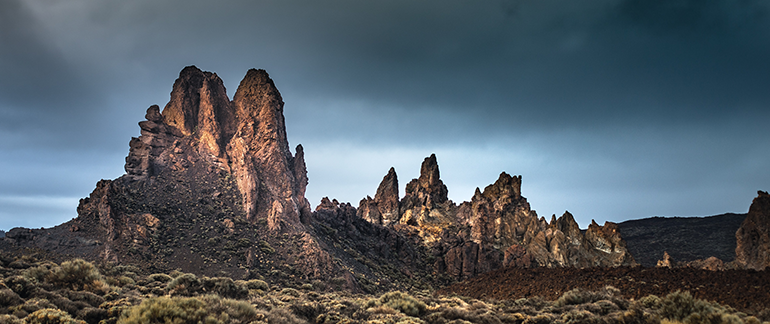
\includegraphics{images/01-image.png}
\caption{Figure caption text is also alt text.}
\end{figure}

Lorem ipsum dolor sit amet, consectetur adipiscing elit. Ut in dolor nibh. Lorem ipsum dolor sit amet, consectetur adipiscing elit. Praesent et augue scelerisque, consectetur lorem eu, auctor lacus. Fusce metus leo, aliquet at velit eu, aliquam vehicula lacus. Donec libero mauris, pharetra sed tristique eu, gravida ac ex. Phasellus quis lectus lacus. Vivamus gravida eu nibh ac malesuada. Integer in libero pellentesque, tincidunt urna sed, feugiat risus. Sed at viverra magna. Sed sed neque sed purus malesuada auctor quis quis massa.

\hypertarget{your-turn-2}{%
\subsubsection*{Your turn!}\label{your-turn-2}}
\addcontentsline{toc}{subsubsection}{Your turn!}

Your browser does not support iframes

\hypertarget{second-section-header-1}{%
\section{Second Section Header}\label{second-section-header-1}}

Lorem ipsum dolor sit amet, consectetur adipiscing elit. Ut in dolor nibh. Lorem ipsum dolor sit amet, consectetur adipiscing elit. Praesent et augue scelerisque, consectetur lorem eu, auctor lacus. Fusce metus leo, aliquet at velit eu, aliquam vehicula lacus. Donec libero mauris, pharetra sed tristique eu, gravida ac ex. Phasellus quis lectus lacus. Vivamus gravida eu nibh ac malesuada. Integer in libero pellentesque, tincidunt urna sed, feugiat risus. Sed at viverra magna. Sed sed neque sed purus malesuada auctor quis quis massa.

\hypertarget{case-study-1}{%
\subsubsection*{Case Study}\label{case-study-1}}
\addcontentsline{toc}{subsubsection}{Case Study}

\hypertarget{box-text}{%
\subsubsection*{Case study title max of forty characters}\label{box-text}}
\addcontentsline{toc}{subsubsection}{Case study title max of forty characters}

Lorem ipsum dolor sit amet, consectetur adipiscing elit. Praesent non magna non nunc auctor eleifend. Etiam fringilla fermentum nisl at volutpat. Duis sodales lorem interdum, posuere neque sollicitudin, malesuada nisl. Sed laoreet commodo dui et cursus. Curabitur vel porta mauris. In lacinia ac ex ac varius. Nullam at vulputate ligula. Nunc sed faucibus urna, eget placerat sapien. Fusce ut lorem a ante congue consequat et sed tortor. Integer neque urna, vehicula at aliquam non, luctus non mi. Pellentesque et massa vehicula, cursus erat id, aliquet sapien. Sed rhoncus vehicula risus, vel aliquam eros porta eget. Etiam maximus, massa in pretium semper, est libero feugiat ipsum, quis tempor nunc libero in nibh. Nunc sollicitudin mattis metus ut rutrum. Donec urna purus, sodales id nibh in, ultricies tincidunt nibh. Proin porta accumsan aliquet.

Cras convallis erat ante, ut tristique est tempor elementum. Nam mollis, ipsum at vehicula vestibulum, est magna finibus nisl, et laoreet metus massa et ipsum. Proin eget eros ac odio euismod volutpat et ac diam. Cras viverra ut libero vel pulvinar. Duis nisi magna, sagittis id ligula ac, efficitur commodo eros. Nulla tincidunt id nulla in lobortis. Sed non mi eu mi fermentum cursus. In elit velit, semper sed gravida at, imperdiet sed nibh. Aliquam quis massa malesuada, venenatis nunc sed, malesuada nulla. Vestibulum malesuada purus ut ex ullamcorper, ut blandit lacus lobortis. Curabitur scelerisque velit justo, quis porttitor purus efficitur ut. Phasellus nec arcu vestibulum, consequat ante id, elementum velit. Proin arcu tortor, cursus vitae sem id, congue semper urna. Integer tempus in est eu consequat. Donec sodales, quam vel finibus faucibus, leo ante dictum quam, id tempus ligula dolor quis erat. Curabitur non elementum sem. Mauris placerat fermentum orci non lacinia. Ut imperdiet dui lectus, ac malesuada felis euismod sed. Nulla non volutpat dui, in suscipit turpis.

Case studies should have at least one image or map (no more than 2 total) and the written length should be around 300 words (shown above). Any references to external literature should by hyperlinked with the Digitial Object Identifier (DOI) permanent URL and \href{https://bookdown.org/yihui/bookdown/citations.html}{entered into the bibliography}. Avoid linking to external resources without a DOI and permanent URL. Contact Paul or try using the Leaflet package in R if you want to add an interactive web map.

\hypertarget{third-section-header-1}{%
\section{Third Section Header}\label{third-section-header-1}}

\href{https://google.com}{This is how we link to something. \{target="\_blank"\} ensures that this link opens in a new window rather than navigating away from the textbook.}

\hypertarget{your-turn-3}{%
\subsubsection*{Your turn!}\label{your-turn-3}}
\addcontentsline{toc}{subsubsection}{Your turn!}

Ask the reader to undertake some activity or exercise. Have them explore data, an interactive tool, a web map. Avoid referencing, relying on, or using external URLs. If it can be built, coded, or hosted by us, then it should be.

Your browser does not support iframes

Lorem ipsum dolor sit amet, consectetur adipiscing elit. Ut in dolor nibh. Lorem ipsum dolor sit amet, consectetur adipiscing elit. Praesent et augue scelerisque, consectetur lorem eu, auctor lacus. Fusce metus leo, aliquet at velit eu, aliquam vehicula lacus. Donec libero mauris, pharetra sed tristique eu, gravida ac ex. Phasellus quis lectus lacus. Vivamus gravida eu nibh ac malesuada. Integer in libero pellentesque, tincidunt urna sed, feugiat risus. Sed at viverra magna. Sed sed neque sed purus malesuada auctor quis quis massa.

\hypertarget{call-out-1}{%
\subsubsection*{Call out}\label{call-out-1}}
\addcontentsline{toc}{subsubsection}{Call out}

This is a call out. Put some important concept or fact in here.

\hypertarget{summary-2}{%
\section{Summary}\label{summary-2}}

Lorem ipsum dolor sit amet, consectetur adipiscing elit. Ut in dolor nibh. Lorem ipsum dolor sit amet, consectetur adipiscing elit. Praesent et augue scelerisque, consectetur lorem eu, auctor lacus. Fusce metus leo, aliquet at velit eu, aliquam vehicula lacus. Donec libero mauris, pharetra sed tristique eu, gravida ac ex. Phasellus quis lectus lacus. Vivamus gravida eu nibh ac malesuada. Integer in libero pellentesque, tincidunt urna sed, feugiat risus. Sed at viverra magna. Sed sed neque sed purus malesuada auctor quis quis massa.

\hypertarget{reflection-questions-1}{%
\subsection*{Reflection Questions}\label{reflection-questions-1}}
\addcontentsline{toc}{subsection}{Reflection Questions}

\begin{enumerate}
\def\labelenumi{\arabic{enumi}.}
\tightlist
\item
  Explain ipsum lorem.
\item
  Define ipsum lorem.
\item
  What is the role of ispum lorem?
\item
  How does ipsum lorem work?
\end{enumerate}

\hypertarget{practice-questions-1}{%
\subsection*{Practice Questions}\label{practice-questions-1}}
\addcontentsline{toc}{subsection}{Practice Questions}

\begin{enumerate}
\def\labelenumi{\arabic{enumi}.}
\setcounter{enumi}{1}
\tightlist
\item
  Given ipsum, solve for lorem.
\item
  Draw ipsum lorem.
\end{enumerate}

Ensure all inline citations are properly referenced here.

\hypertarget{data-integration}{%
\chapter{Chapter Title}\label{data-integration}}

\textbf{Frogs}, This chapter is about Frogs

\hypertarget{learning-objectives-3}{%
\subsubsection*{Learning Objectives}\label{learning-objectives-3}}
\addcontentsline{toc}{subsubsection}{Learning Objectives}

\begin{enumerate}
\def\labelenumi{\arabic{enumi}.}
\tightlist
\item
  Objective one
\item
  Objective two
\item
  Objective three
\end{enumerate}

\hypertarget{key-terms-3}{%
\subsection*{Key Terms}\label{key-terms-3}}
\addcontentsline{toc}{subsection}{Key Terms}

Ipsum lorem, Phasellus, sollicitudin, finibus

16.1 Problems with data integration\\
16.1.1 Data types, sources, formats\\
16.1.2 Datums, extents, scales\\
16.1.3 Data resolutions\\
16.2 Integrating vector and raster data Chris Liang
16.2.1 Rasterization\\
16.2.2 Vectorization\\
16.2.3 Features from rasters\\
16.2.4 Rasters to features\\
16.2.5 Smoothing\\
16.2.6 Simplifying\\
16.3 Spatial data errors\\
16.3.1 Accuracy Attribute errors
16.3.2 Precision\\
16.3.3 Systematic errors Recall GNSS errors
16.3.4 Random errors\\
16.3.5 Quantifying spatial errors RMSE, Euclid's distance

  \bibliography{book.bib}

\end{document}
